\chapter[Resultados]{Resultados}

Com a inclusão dos sensores no sistema, obtemos a coleta dos dados que são considerados importantes para as mudanças físicas que irão ocorrer no ambiente virtual, bem como a produção de sensações no usuário de forma que o mesmo tenha um experiência semelhante a andar de bicicleta na rua. Os seguintes dados estão sendo coletados: velocidade e direção a qual o guidão é movimentado.
% e nível da bateria para o sistema de realimentação.

Os dados da velocidade serão apresentados ao atleta para que ele tenha consciência do seu desempenho. O sinal do sensor de direção do guidão fará com que haja uma alteração no ambiente virtual, ou seja, dependendo da angulação do guidão, o usuário terá a sensação de que está fazendo uma curva. Outro dado importante é que quando houver uma subida no percurso do ambiente virtual o usuário terá maior dificuldade ao pedalar, como se realmente estivesse subindo um morro, por exemplo.

Por meio destas características, espera-se simular um ambiente que seja tão próximo quanto possível da realidade de forma a tornar atividades físicas, como o \textit{spinning}, algo menos monótono já que o atleta não se desloca e apresentar dados que possam melhorar seu rendimento. Outro resultado interessante é realizar a comparação do nível de iteratividade do sistema com uma situação real e analisar como o usuário se comporta em ambos os ambientes. Isso é interessante para atletas de alto nível pois simular o percurso de uma prova e ter conhecimento das reações do corpo naquele ambiente é de fundamental importância para um bom desempenho.

Uma das medidas adotadas pela equipe para a produção do produto foi  a busca pela conservação da estrutura original da bicicleta, no intuito que o produto possa ser oferecido como um pacote sem a inclusão da bicicleta, permitindo que com algumas peças e a remoção da roda traseira a bicicleta possa ser adaptada para o uso do produto.

\section {Ambiente virtual}

\subsection{ Melhora da Usabilidade e Imersão no ambiente virtual }

Após o término do desenvolvimento do ambiente virtual, viu-se a necessidade de uma melhora na usabilidade e imersão, por parte do usuário, no ambiente virtual. Durante os testes realizados pela equipe foram encontrados alguns problemas como: a grande distância entre os pontos chave do ambiente virtual, onde o usuário deveria de locomover por quilômetros para atravessar todo o mapa desenvolvido; a grande largura das trilhas, que acabavam que não guiavam muito bem o usuário durante o percurso; o fato do usuário poder sair dos limites da trilha proposta e se adentrar em lugares não planejados e projetados para isso; alguns objetos do ambiente eram desproporcionais entre si, sendo alguns objetos muito grandes e outros muito pequenos; as informações apresentadas para o usuário, como velocidade, não estavam em um local adequado.

Tendo em vista as dificuldades anteriormente encontradas para a utilização do ambiente virtual, foram feitas algumas melhorias a fim de maximizar a boa experiência do usuário no contexto do Bike-X. A seguir, são apresentadas as soluções adotadas:

O ambiente virtual como um todo foi reduzido, para que o usuário consiga realizar todo o percurso em um tempo e uma distância aceitáveis, sem valores absurdos. A figura \ref{fig:mapaReduzido}, mostra a visão superior do mapa desenvolvido para o ambiente virtual.

\begin{figure}[h]
  \centering
  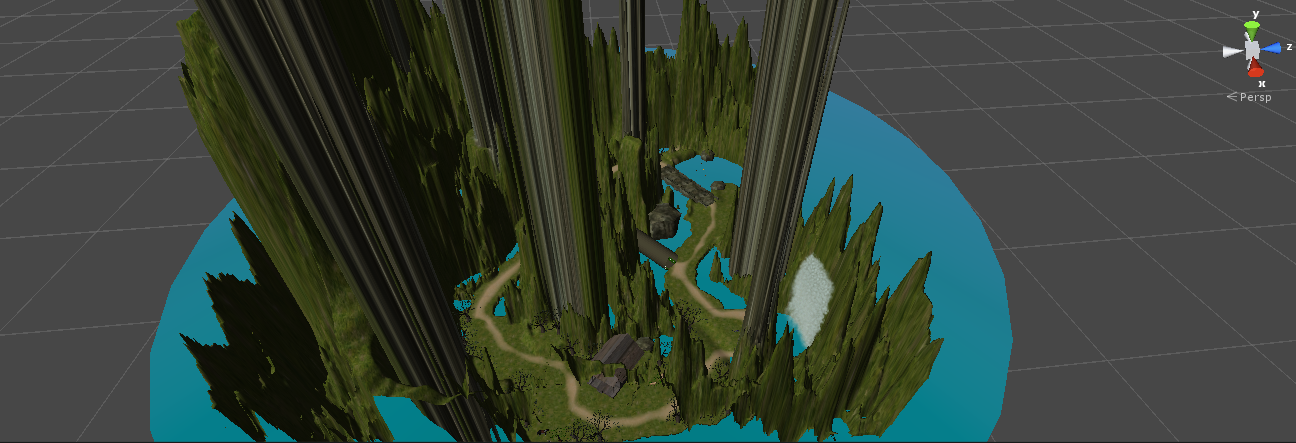
\includegraphics[width=1.0\textwidth]{figuras/mapaReduzido}
  \caption{Visão superior do mapa reduzido}
  \label{fig:mapaReduzido}
\end{figure}

As trilhas se tornaram mais estreitas, norteando de uma melhor maneira o usuário no decorrer do percurso. Além disso, foram adicionados alguns objetos adjacentes ao percurso a fim de melhorar a experiência do usuário, como os animais ilustrados na figura \ref{fig:animaisPista}. Os animais apresentados apresentavam problemas de proporção com o resto do ambiente virtual, com isso, a escala de tamanho dos mesmos foi reduzida.

\begin{figure}[h]
  \centering
  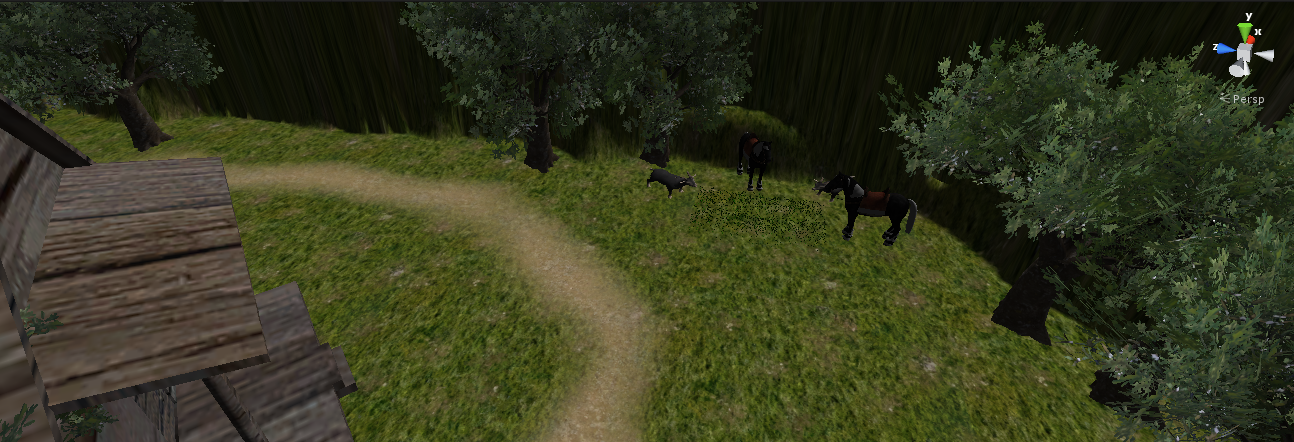
\includegraphics[width=1.0\textwidth]{figuras/animaisPista}
  \caption{Visão da trilha com animais adjacentes}
  \label{fig:animaisPista}
\end{figure}

Como pode ser visto nas figuras \ref{fig:blocosPercurso} e \ref{fig:blocosColisao}, foram criados vários blocos de colisão ao redor de toda a trilha para que o usuários não possa atingir lugares inadequados, como a água. Essa solução foi implementada utilizando planos invisíveis para o usuário, que o impedirá de ultrapassar determinados limites. A utilização de planos foi a forma mais fácil, identificada pela equipe, de se contornar o problema enfrentado.

\begin{figure}[h]
  \centering
  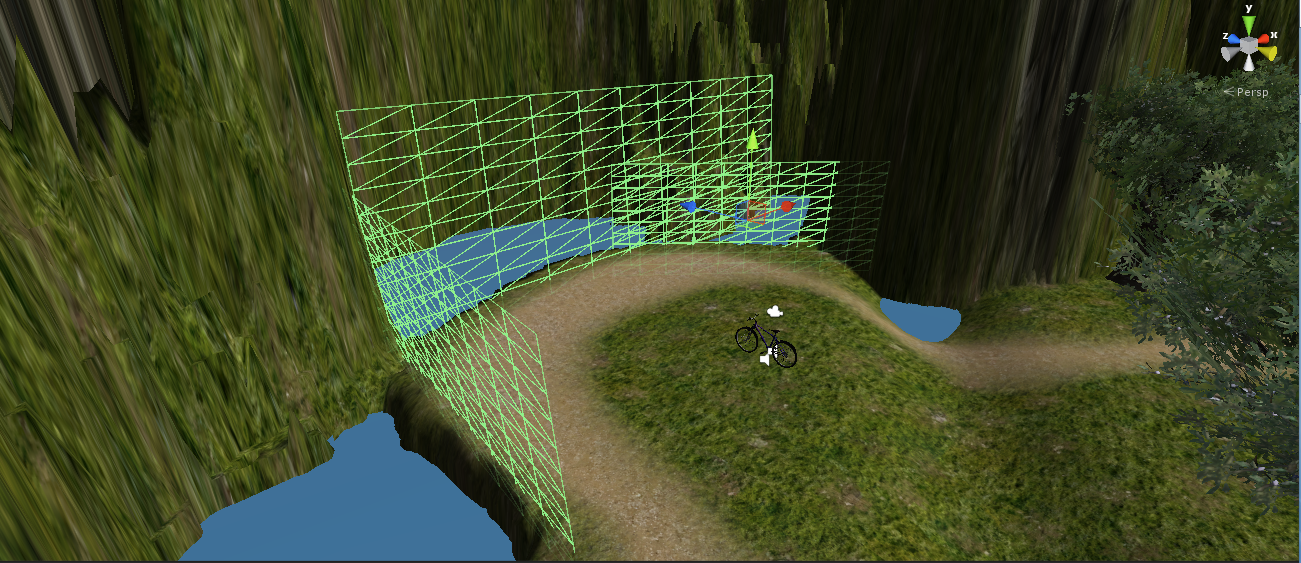
\includegraphics[width=1.0\textwidth]{figuras/blocosColisao}
  \caption{Blocos de Colisão}
  \label{fig:blocosColisao}
\end{figure}

\begin{figure}[h]
  \centering
  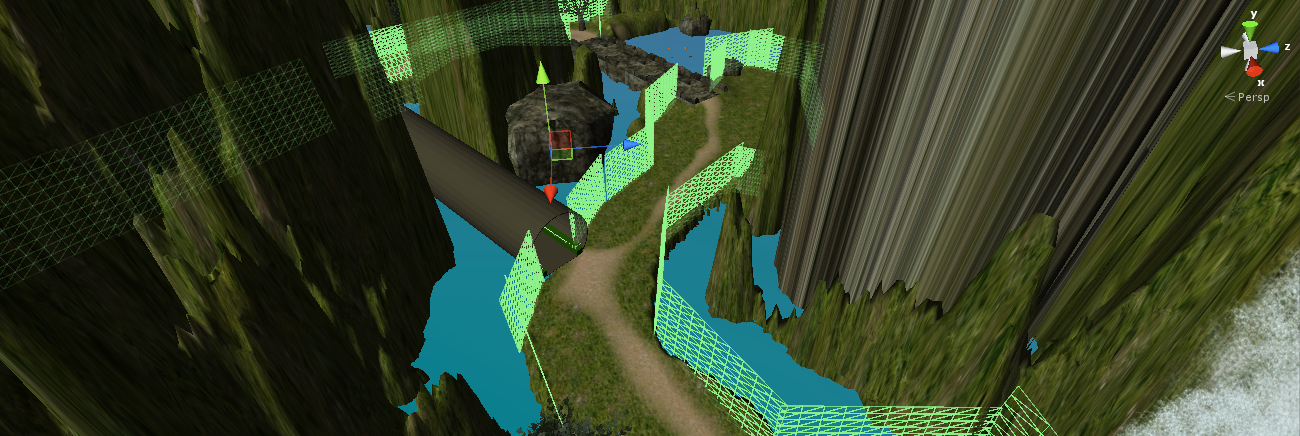
\includegraphics[width=1.0\textwidth]{figuras/blocosPercurso}
  \caption{Blocos de Colisão no decorrer do percurso da trilha}
  \label{fig:blocosPercurso}
\end{figure}

Depois da criação dos blocos de colisão para impedir que o usuário ultrapasse locais indevidos foi acrescentado ao ambiente \textit{ MeshRenderCollider } de colisões de objetos nas pontes, pedras, animais, árvores e na casa, assim quando o usuário tentar colidir com uma casa ou com um animal , ou ao mesmo atravessar a ponte ou o túnel ele não irá passar por dentro do mesmo e sim por cima, permitindo a travessia, como pode ser visto nas figuras \ref{fig:bridgePosition}, \ref{fig:newTunnel} e \ref{fig:animalsCollider}.

\begin{figure}[h]
  \centering
  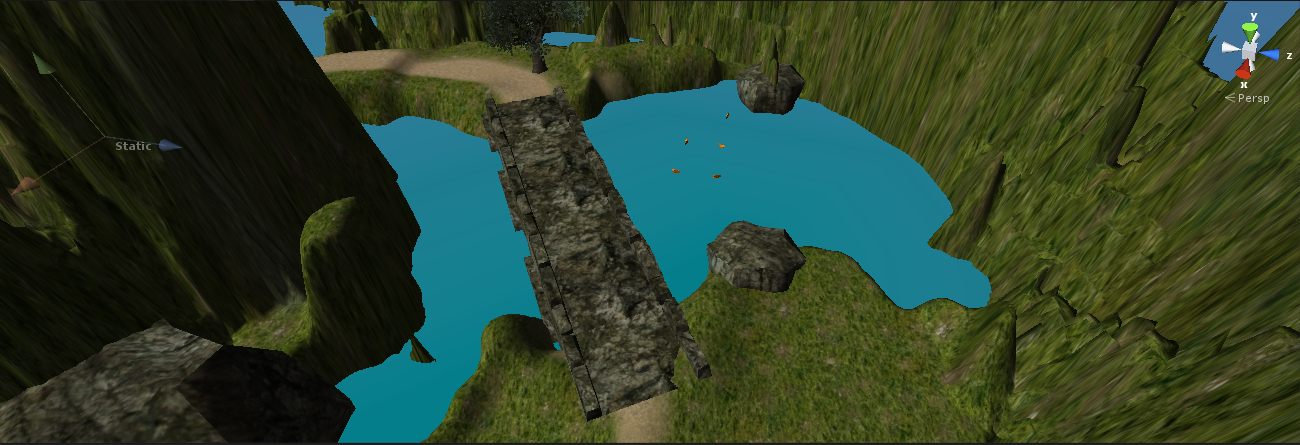
\includegraphics[width=1.0\textwidth]{figuras/bridgePosition}
  \caption{Ponte utilizada no ambiente virtual}
  \label{fig:bridgePosition}
\end{figure}

\begin{figure}[h]
  \centering
  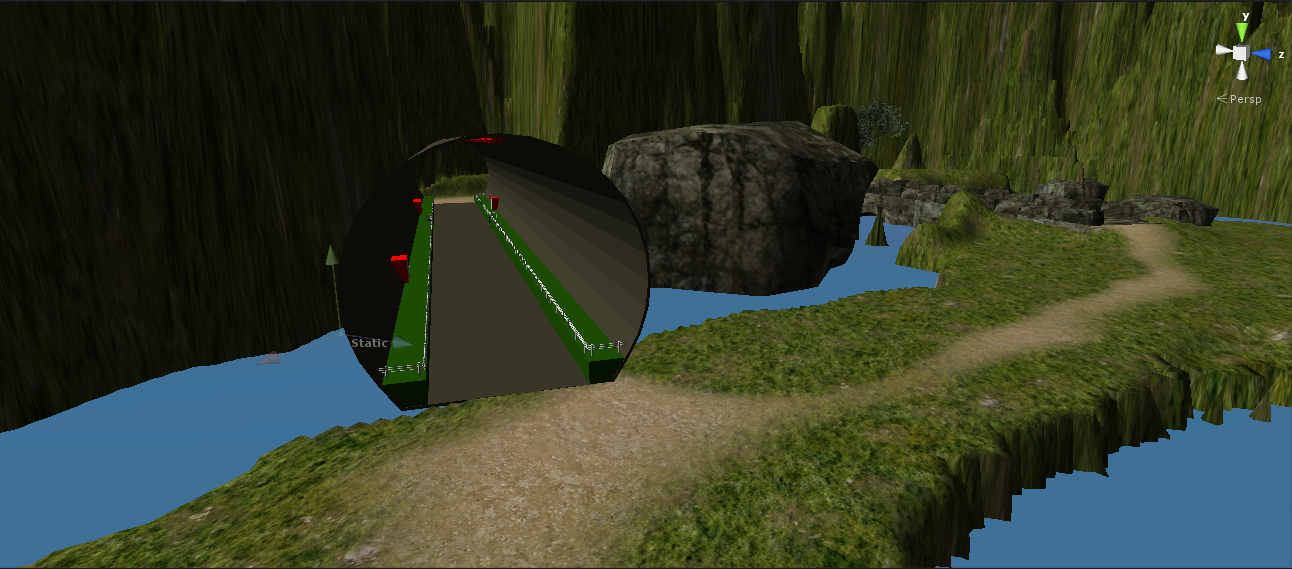
\includegraphics[width=1.0\textwidth]{figuras/newTunnel}
  \caption{Túnel utilizado no ambiente virtual}
  \label{fig:newTunnel}
\end{figure}

\begin{figure}[h]
  \centering
  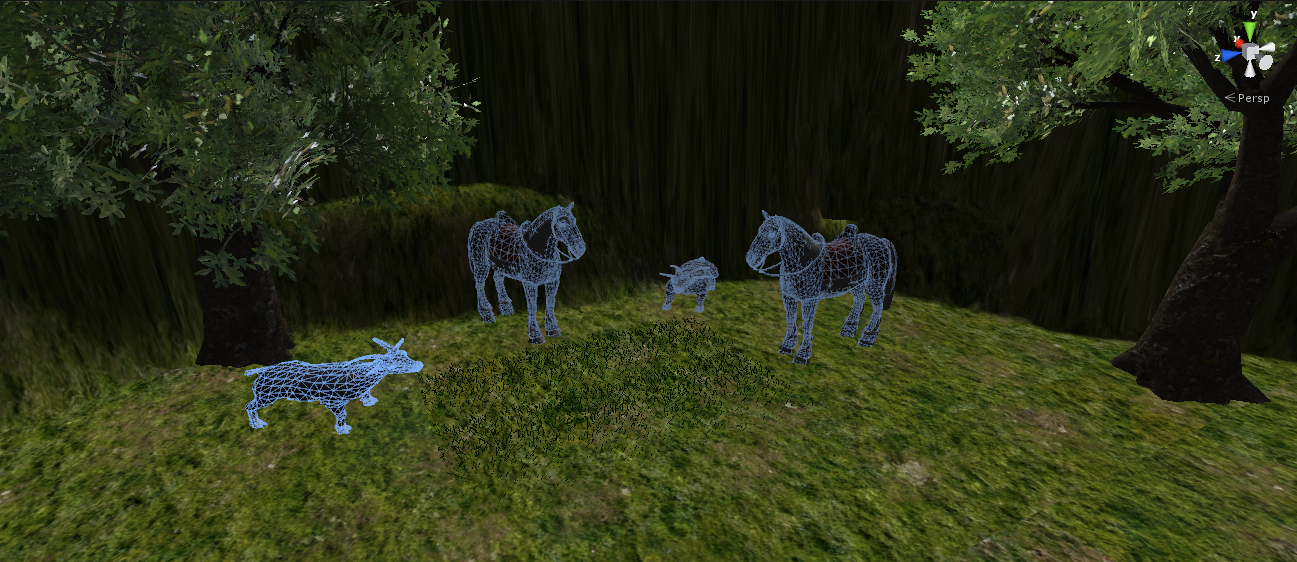
\includegraphics[width=1.0\textwidth]{figuras/animalsCollider}
  \caption{Colisão nos animais adjacentes a trilha}
  \label{fig:animalsCollider}
\end{figure}

Para melhorar ainda mais a experiência do usuário foram adicionados sons de natureza no ambiente virtual, como o som da cachoeira que foi adicionada ao percurso (figura \ref{fig:waterFallPosition}) e de corrente de água ao atravessar a ponte.

\begin{figure}[h]
  \centering
  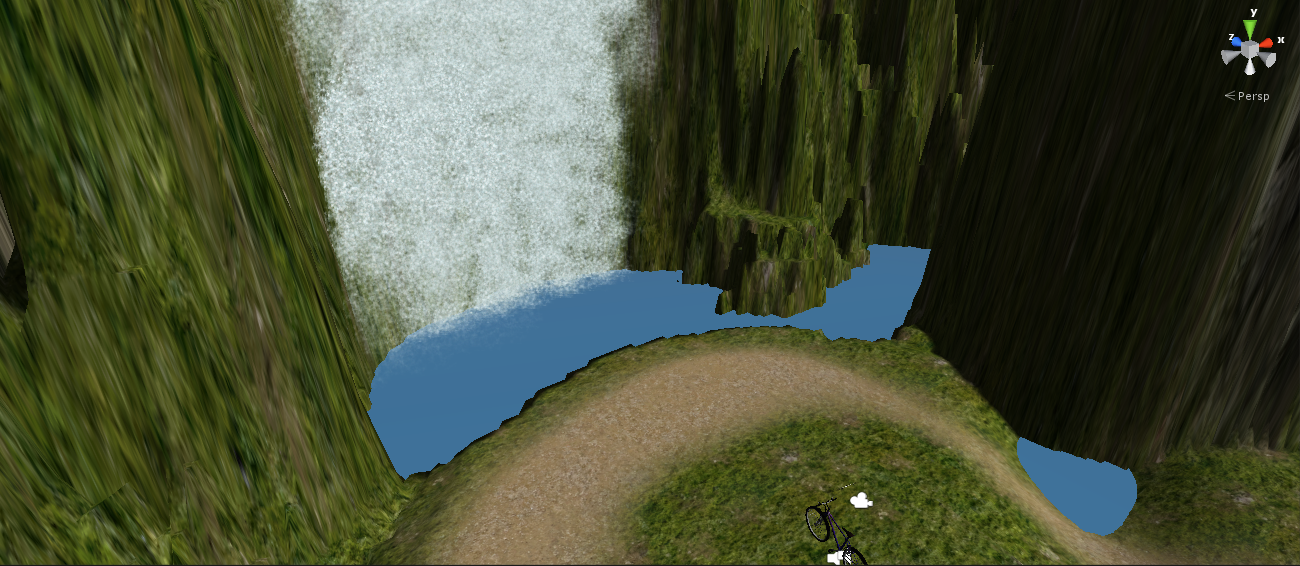
\includegraphics[width=1.0\textwidth]{figuras/waterFallPosition}
  \caption{Cachoeira presente no decorrer da trilha}
  \label{fig:waterFallPosition}
\end{figure}

A principal dificuldade encontrada pela equipe foi em como apresentar as informações para o usuário na tela sem comprometer a interação com o ambiente virtual. Preferiu-se então apresentar de uma maneira bem simples, através de uma caixa de diálogo no canto superior direito da tela, como pode ser visto na figura \ref{fig:improvedInterface}, ao invés de apenas adicionar as informações no centro da tela.


\begin{figure}[h]
  \centering
  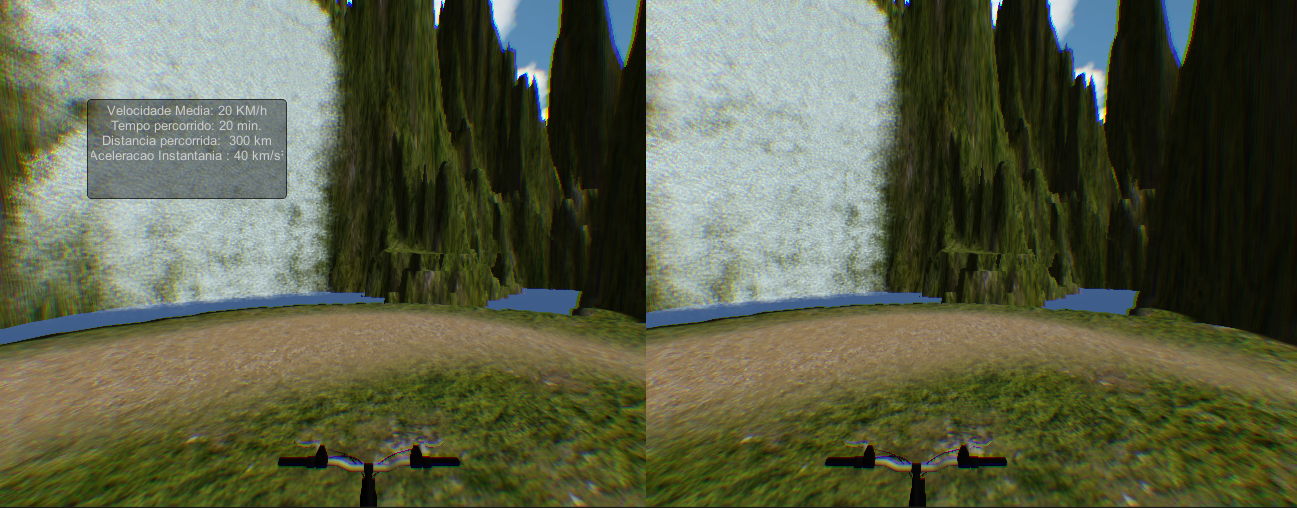
\includegraphics[width=1.0\textwidth]{figuras/improvedInterface}
  \caption{\textit{Interface} com o usuário para apresentação de informações}
  \label{fig:improvedInterface}
\end{figure}



\chapter{Manual do Produto} % (fold)
\label{cha:manual_do_produto}
 
O trecho a seguir descreve o processo recomendado pela equipe para o uso do produto, assim como os cuidados que devem ser tomados com o manuseio.

\section{Modo de Uso} % (fold)
\label{sec:modo_de_uso}

\begin{enumerate}
	\item Verifique se a aplicação já esta em funcionamento com o auxilio da tela secundaria (notebook/monitor).
	\item Posicione-se sobre a bicicleta. Verifique se a mesma se mantem  estável com o seu peso. Para mais informações sobre os valores para qual este produto foi projetado, verificar \autoref{dados_usuario}.
	\item Imerja-se na realidade virtual com o \gls{rift}.
	\item Após o uso do equipamento, remova o \gls{rift} e espere de 15 a 30 segundos antes de tentar desmontar da bicicleta\footnote{Devido a alta imersão, é recomendado um tempo para se acostumar novamente com a realidade antes de realizar movimentos bruscos.}.
\end{enumerate}

\section{Precauções} % (fold)
\label{sec:precau_es}

\begin{description}
	\item [Não tente desmontar da bicicleta utilizando o gls{rift}] $-$ Ao utilizar o \gls{rift}, a imersão proporcionará uma perca da noção de espaço e posição da realidade. Tentar se movimentar na realidade visualizando o ambiente virtual é extremamente desencorajador.
	\item [Não grite] $-$ A imersão no ambiente virtual causa uma perca de contato com a realidade, lembre-se disto antes de tentar se comunicar com aqueles que te assistem.
	\item [Evite balançar muito na bicicleta ou ficar em pé nela] $-$ Apesar de cálculos terem sido feitos no intuito de manter a bicicleta o mais estável possível ao chão, o produto ainda é passível de tombamento quando exposto a determinados momentos angulares.
	\item [Divirta-se] $-$ Mesmo tendo como objetivo apresentar uma alternativa para a pratica de atividades físicas em ambientes fechados, o projeto busca oferecer também entretenimento ao usuário.
	\item [Mantenha o produto] $-$ Evite reajustar os sensores, a altura do guidão ou do banco. Por ser um protótipo, o produto ainda não oferece um amplo grau de personalização. Tentar configurar o equipamento sem o devido conhecimento do produto pode vir a danifica-lo ou  ao comprometimento dos sinais adquiridos para controle do ambiente.
\end{description}
